\section{Diskussion}

\subsection{Teststrecke 1}

Durch die implementierten Funktionen wurde ersichtlich, dass bei der Berechnung der Zeit bisher die Steigung als entscheidender Faktor nicht betrachtet wurde.

\begin{figure}[H]
\centering
\begin{subfigure}{0.80\textwidth}
\centering
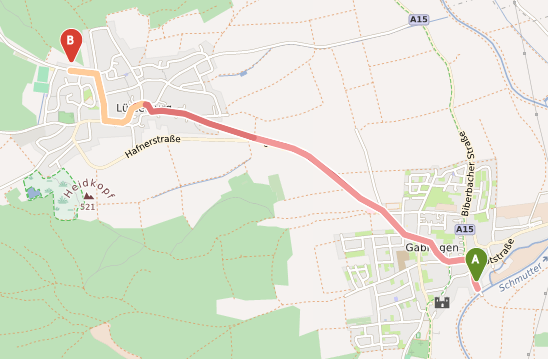
\includegraphics[width = \textwidth]{../media/Fahrt1_Steep.png} \\
\caption{Strecke 1 mit Steigung}
\label{fig:steig}
\end{subfigure}

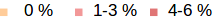
\includegraphics[width =0.25 \textwidth]{../media/legend2.png} \\

\begin{subfigure}{ \textwidth}
\centering
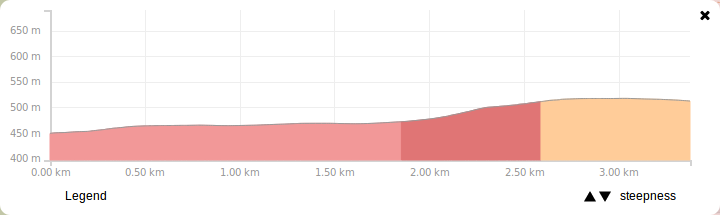
\includegraphics[width = \textwidth]{../media/Fahrt1_Profile.png} \\
\caption{Höhenprofil der ersten Strecke}
\label{profile}
\end{subfigure}
\caption[Einfluss der Steigung auf der ersten Teststrecke]
{\centering Einfluss der Steigung auf der ersten Teststrecke
\par\justifying\scriptsize
Die Steigung der Strecke ist auf der ersten Testfahrt abgebildet (a).
Auch das Höhenprofil (b) für die Strecke zeigt einen signifikanten Anstieg.
Dieser wurde bisher nicht mit einkalkuliert, ist aber für ein Löschfahrzeug aufgrund des hohen Gewichts relevant.
}
\label{steig}
\end{figure}

Auf der ersten Teststrecke muss das Löschfahrzeug insgesamt einen Höhenunterschied von ungefähr 70 Metern überwinden (Abb.~\ref{profile}).
Über die Hälfte der Distanz besteht dabei eine Steigung von 1-3$\%$ und auf einem Viertel der Strecke sogar eine Steigung von 4-6$\%$.
Ein Fahrzeug dieser Gewichtsklasse kann auf dieser Strecke folglich nicht die für den größten Teil dieses Anstiegs geltende Maximalgeschwindigkeit von 80 km/h erreichen.


Darüber hinaus liegen auf der Strecke, im inneren Lützelburgs, einige langgezogene, aber dennoch enge Kurven (Abb.~\ref{fig:curve}).
Auch hier kann das Löschfahrzeug nicht die gegebene Geschwindigkeit beibehalten und muss abbremsen.
Diese Kurven werden allerdings vom Löschfahrzeug-Profil nicht als Abbiegung erkannt, da der Winkel zwischen den Segmenten zu groß ist.
Daher absolviert das Profil diesen Streckenabschnitt in geringerer Zeit, als das echte Fahrzeug.

\begin{figure}[htb]
\centering
\caption[Teststrecke 1 -- Unregistrierte Abbiegungen]
{\centering Teststrecke 1 -- Unregistrierte Abbiegungen
\par\justifying\scriptsize
Auf der Abbildung sind enge Kurven in der Ortsmitte von Lützelburg zu sehen.
Diese können nicht mit der erlaubten Geschwindigkeit gefahren werden, wurden jedoch nicht als Abbiegung registriert, da der Öffnungswinkel zu groß ist.
}
\label{fig:curve}
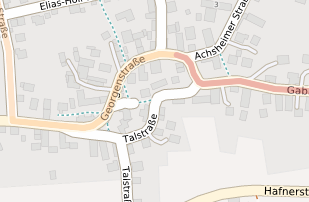
\includegraphics[width = 0.50 \textwidth]{../media/Fahrt1_curve.png} \\
\end{figure}

Weiterhin wurde für jede der drei Fahrten beobachtet, dass auf den Segmenten mit Maximalgeschwindigkeit (80 km/h) das Profil ebenfalls konstant ein paar Sekunden gegenüber der Testfahrt gutmachen kann.
Die Erklärung dafür ist, dass das Löschfahrzeug die angegebene Maximalgeschwindigkeit nicht komplett erreichen kann.
Auch wenn die Angabe mit der Geschwindigkeitsanzeige übereinstimmt, ist die effektive Geschwindigkeit geringer.

Die Zeitdifferenzen aus Tabelle \ref{tab:all} zeigen: das Profil fährt dem echten Fahrzeug mit der derzeitigen Gewichtung über die ganze Strecke voraus.
Wenn die genannten Faktoren der Steigung, der nicht mit einberechneten schärferen Kurven und der Maximalgeschwindigkeit mit einbezogen werden, ist ein Ergebnis von etwa 5 Minuten zu erwarten.

\subsection{Teststrecke 2}

Da die 2. Strecke nur in der Ebene verläuft, sind keine Abweichungen durch die Steigung zu erwarten.
Die Differenzzeiten betragen für alle fünf Wegpunkte ungefähr 10 Sekunden.
Auffallend ist der Sprung vom 3. zum 4. Wegpunkt, bei welchem das Profil 14 Sekunden aufholt.
Nach einer genaueren Betrachtung dieses Segments stellte sich heraus, dass hier eine enge Unterführung durchfahren werden musste, auf die eine durch die Topologie unübersichtliche Kurve folgt (Abb.~\ref{fig:traintunnel}).
Daher kam es auf der Fahrt zu Verzögerungen, welches das Aufholen des Profils gegenüber der Testfahrt erklärt.

\begin{figure}[htb]
\centering
\caption[Teststrecke 2 -- Unterführung]
{\centering Teststrecke 2 -- Unterführung
\par\justifying\scriptsize
Die Verzögerung durch diese enge Unterführung und die danach folgende, unübersichtliche Kurve auf der zweiten Teststrecke, wurde durch das Profil für Löschfahrzeuge nicht berücksichtigt.
}
\label{fig:traintunnel}
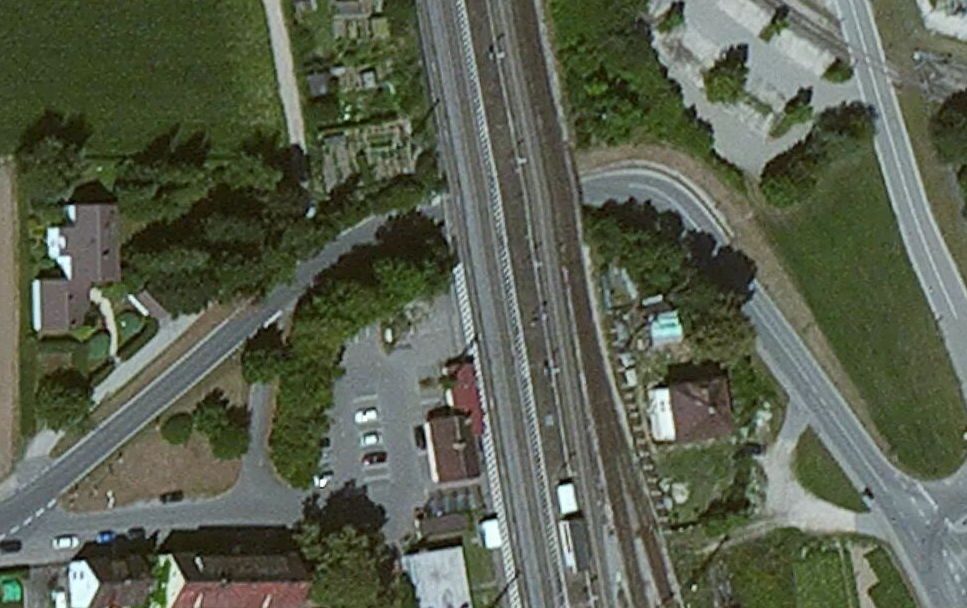
\includegraphics[width = 0.70 \textwidth]{../media/traintunnel.png} \\
\end{figure}


\subsection{Teststrecke 3}

Bei den Ergebnissen der 3. Strecke (Tab. \ref{tab:all}) ist das Profil bereits nach dem ersten Wegpunkt um mehr als 10 Sekunden zu langsam.
Bis zum Zwei-Minuten-Wegpunkt wird dieser Rückstand fast verdoppelt.
Nach genauerer Überprüfung der Durchschnittsgeschwindigkeiten stellte sich heraus, dass der Weg hier durch eine 30er-Zone führt.
Allerdings wird diese nicht mit den erwarteten 50 km/h, sondern nur mit den durch den \texttt{maxspeed} Tag festgelegten 30 km/h durchfahren.
Offensichtlich ist dies ein Fehler im Backend welcher behoben werden muss.

\begin{figure}[htb]
\centering
\caption[Teststrecke 3 -- Tempo-30-Zone]
{\centering Teststrecke 3 -- Tempo-30-Zone
\par\justifying\scriptsize
Auf der dritten Teststrecke befindet sich eine 30er-Zone welche von dem Profil für Löschfahrzeuge noch nicht erkannt wird.
}
\label{fig:temp30}
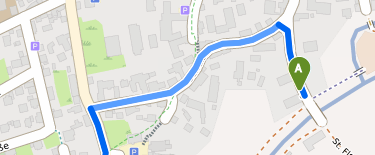
\includegraphics[width = 0.60 \textwidth]{../media/Fahrt3_temp30.png} \\
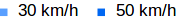
\includegraphics[width = 0.20 \textwidth]{../media/legend3.png} \\
\end{figure}

Die anfängliche 30er-Zone ist fast 350m lang.
Diese Strecke kann mit 50 km/h in 25,2 Sekunden und mit 30 km/h in 42 Sekunden durchfahren werden.
Wird die Differenz von 16.8 Sekunden von den bisherigen Abweichungen für die 3. Fahrt abgezogen, werden die neuen Werte aus Tabelle \ref{tab:new3} erhalten.

\begin{table}[htb]
\centering
\caption{Teststrecke 3 -- neue Fahrzeit}
\label{tab:new3}
\begin{tabular}{|l|r|r|}
\hline
Wegpunkt & Fahrzeit & Abweichung \\ \hline 
1$min$ & 58.2$s$\footnote{Zum ersten Wegpunkt beträgt die Strecke nur 260m, weshalb hier nur 12.6 Sekunden abgezogen werden} & -1.8$s$  \\
2$min$ & 122.6$s$ & +2.6$s$  \\
3$min$ & 173.2$s$ & -6.8$s$  \\
4$min$ & 238.4$s$ & -1.6$s$  \\
5$min$ & 296.1$s$ & -3.9$s$  \\
\hline
\end{tabular}
\end{table}

Vor der 2-Minuten-Marke beginnt eine Überlandstraße, die bis kurz vor Holzhausen (zwischen Marker 3 und 4) reicht.
Das sind 56$\%$ der Gesamtstrecke.
Wie bei der Diskussion der 1. Fahrt bereits erwähnt ist zu erwarten, dass die Maximalgeschwindigkeit von 80km/h zu hoch angesetzt ist, welches den leichten Vorsprung zur 3-Minuten-Marke erklärt.

\begin{figure}[H]
\centering
\begin{subfigure}{0.49\textwidth}
\centering
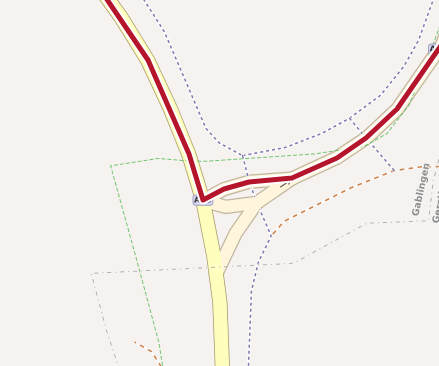
\includegraphics[width = 0.80\textwidth]{../media/Fahrt3_Turn.png} \\
\caption{Abbiegung auf \gls{osm}-Datenebene}
\label{fig:turnosm}
\end{subfigure}
\begin{subfigure}{0.49\textwidth}
\centering
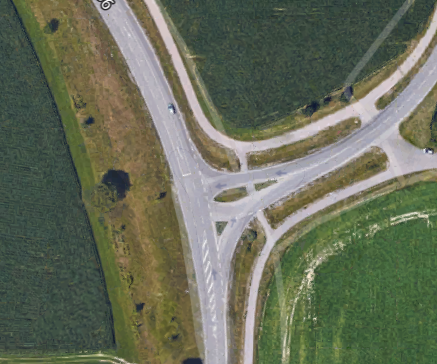
\includegraphics[width = 0.80\textwidth]{../media/Fahrt3_actualturn.png} \\
\caption{Eigentliche Abbiegung}
\label{fig:turnworld}
\end{subfigure}
\caption[Teststrecke 3 -- Vergleich einer Abbiegung]
{\centering Teststrecke 3 -- Vergleich einer Abbiegung
\par\justifying\scriptsize
Diese Abbiegung befindet sich zwischen Gablingen und Holzhausen.
Die Kurve ist in OSM im rechten Winkel eingetragen (a).
In Wirklichkeit ist der Öffnungswinkel der Kurve allerdings größer (b).
}
\label{fig:turn}
\end{figure}

Zwischen Punkt 3 und 4 fällt das Löschfahrzeug-Profil um fünf Sekunden zurück.
Zwischen diesen Punkten befindet sich eine Abbiegung, die deutlich schneller als andere Kurven gefahren werden kann.
Abbildung \ref{fig:turn} zeigt einen Vergleich dieser Abbiegung zwischen den \gls{osm} Daten (Abb.~\ref{fig:turnosm}) und der eigentlichen Straße (Abb.~\ref{fig:turnworld}).
Es ist zu erkennen, dass die Abbiegung um einiges ''weicher'' ist, als die Daten beschreiben.
Daher konnte das Löschfahrzeug gegenüber dem Profil hier Zeit gewinnen.

Schließlich zeigte auch diese Strecke, nach einer Untersuchung des Höhenprofils, einen Anstieg auf den letzten 150 Metern um 7-9$\%$(Abb.~\ref{fig:profile2}), der noch nicht mit einberechnet wird, und dem Löschfahrzeug-Profil somit einen kleinen Vorsprung gibt.

\begin{figure}[htb]
\centering
\caption{Teststrecke 3 -- Höhenprofil}
\label{fig:profile2}
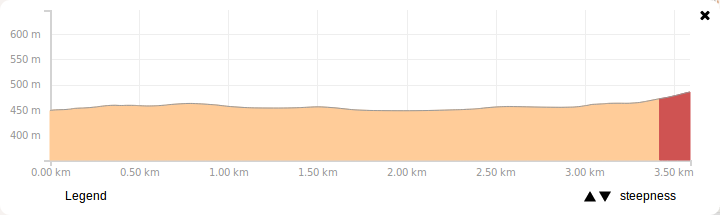
\includegraphics[width = 0.90 \textwidth]{../media/Fahrt3_Profile.png} \\
\end{figure}


\subsection{Benötigte Änderungen}

Wie aus den vorliegenden Analysen hervorgeht, müssen einige Änderungen vollzogen werden, damit das Profil realistischere Ergebnisse berechnet.\par
\begin{itemize}
\item 30er Zonen werden noch nicht richtig erkannt.
\item Die Steigung muss berücksichtigt werden.
\item Abbiegevorgänge innerhalb von Segmenten (Abb.~\ref{fig:curve}), an Pillar Nodes, werden bisher nicht berücksichtigt und müssen mit einbezogen werden.
\item Die Zeit für einen Abbiegevorgang sollte sowohl anhand des effektiven Winkels als auch anhand der Geschwindigkeiten des vorherigen und folgenden Wegsegmentes bestimmt werden.
Ansätze hierfür wurden bereits entwickelt (siehe Source Code), wurden allerdings noch nicht getestet.
\item Für die Penalties muss die Zeit, sofern vorhanden, aus der eigentlichen Beschleunigung und, falls nicht vorhanden, zum Beispiel aus dem Gewicht des Fahrzeugs berechnet werden.
Dadurch können einfacher spezifische Fahrzeugprofile erstellt und getestet werden.
Da das \texttt{AccelerationWeighting} sowohl für das Löschfahrzeug, als auch für allgemeine Einsatzfahrzeuge benutzt wird, erhalten diese bisher die gleichen Penalties.
\item Weiterhin muss für Einbahnstraßen, die in Gegenrichtung durchfahren werden, ein Penalty (ca. *0.9) gesetzt werden, da diese oft nicht mit der selben Geschwindigkeit durchfahren werden können, wie in der eigentlichen Fahrtrichtung (auch wenn es erlaubt ist).
Auf diese Weise kann außerdem ein Routing auf der Gegenfahrbahn, lediglich für den Gewinn von wenigen Sekunden, verhindert werden.
Darüber hinaus werden damit bevorzugt vorhandene Parallelstraßen benutzt.
\end{itemize}